\documentclass[a4paper, 10pt, oneside]{article} % A4 paper size, default 11pt font size and oneside for equal margins
\usepackage[utf8]{inputenc} % Required for inputting international characters
\usepackage[T1]{fontenc} % Output font encoding for international characters
\usepackage{hyperref}
\usepackage[italian]{babel}
\usepackage{graphicx}
\usepackage{titlesec}
\usepackage[titles]{tocloft}
\usepackage{amsmath,amsfonts,amssymb}
\usepackage{multirow}
\usepackage{verbatim}
\usepackage{listings}
\usepackage{xcolor}
\usepackage[a4paper,top=3cm,left=3cm,right=3cm,bottom=3cm]{geometry}
\usepackage{markdown}
\usepackage{array}
\usepackage{fancyhdr}
\usepackage{float}




\begin{document}

\pagestyle{fancy}
	\fancyhf{}
	\fancyhead[L]{Progetto -- Basi di Dati}
	\fancyhead[C]{}
	\fancyhead[R]{\textit{"Sistema di prenotazione per le aule universitarie"}}
	\renewcommand{\headrulewidth}{0.4pt}
	\fancyfoot[L]{A. A. 2022-2023}
	\fancyfoot[C]{\thepage}
	\fancyfoot[R]{Giovanni de Maria -- IN0500952}
	\renewcommand{\footrulewidth}{0.4pt}

	\thispagestyle{empty}	
{
		\centering 
	
	\vspace*{\baselineskip} % White space at the top of the page
	
	\textsc{Università degli Studi di Trieste - Dipartimento di Ingegneria e Architettura}
	\bigskip\bigskip
	
	\rule{\textwidth}{1.6pt}\vspace*{2pt} % Thick horizontal rule
	
	\vspace{0.75\baselineskip} % Whitespace above the title
	
	{\LARGE Progetto -- Basi di Dati\\
 \textit{"Sistema di prenotazione per le aule universitarie"}} % Title
 
	
	\vspace{0.75\baselineskip} % Whitespace below the title6
	
	\rule{\textwidth}{1.6pt}\vspace*{2pt} % Thick horizontal rule

	\vspace{2\baselineskip} % Whitespace after the title block
	
	Giovanni de Maria \\
	\medskip
	Matricola: IN0500952\\
	\bigskip
	Anno Accademico 2022-2023\\
    \bigskip
    \url{https://github.com/giovannidemaria/DBProjectUNITS}
	

	}

\tableofcontents
\newpage
\section{Descrizione del progetto e scopi d'uso}

Il progetto si propone di sviluppare un sistema di prenotazione di aule universitarie che permetta la gestione simultanea di più università. Sarà possibile gestire informazioni sui corsi e sugli eventi che si svolgono all'interno delle aule e di assegnare una persona responsabile per ogni prenotazione o evento.\\

Il sistema sarà gestito dal personale amministrativo di ogni università che avrà accesso alle funzionalità di aggiunta, modifica e cancellazione di informazioni sulle aule, sui corsi, sugli eventi e sulle persone che prenotano. Gli utenti potranno accedere al sistema attraverso un sito web senza autenticazione che consentirà loro di visualizzare le informazioni sulle aule disponibili, le informazioni sui corsi e sugli eventi in corso o programmati.


\section{Entità e relazioni}

\begin{figure}[h]
  \centering
\includegraphics[width=1.0\textwidth]{Diagramma\_Entity\_Relationship\_Progetto2705.png}
  \caption{Schema entity - relationship}
  Gli identificatori sono stati evidenziati in ciano.\\
\end{figure}

\newpage


\begin{table}[H]
\begin{tabular}{m{2.25cm} | m{6cm}| m{3.5cm} | m{1.5cm} }

\textbf{Entità} & \textbf{Descrizione} & \textbf{Attributi} & \textbf{Identificatore}\\

\hline

Università  & Rappresenta un'Università& id\_università, nome, indirizzo & id\_università\\

\hline

Edificio   & Rappresenta un edificio dell'Università & id\_edificio, nome, indirizzo, id\_università & id\_edificio\\

\hline

Utente & Rappresenta l'utente che si prende la responsabilità delle singole prenotazioni. Può essere un docente, uno studente o un esterno.& id\_utente, nome, cognome, email, id\_università & id\_utente \\

\hline

Corso & Rappresenta un corso dell'Università & id\_corso, nome, descrizione, id\_utente, id\_università & id\_corso\\

\hline

Aula & Rappresenta una classe all'interno di un Edificio & id\_aula, nome, capacità, id\_edificio,id\_edificio, id\_università & id\_aula \\

\hline

Prenotazione & Rappresenta la prenotazione di un'Aula & id\_prenotazione, id\_aula, data, ora\_inizio, ora\_fine, id\_corso, descrizione, id\_università & id\_prenotazione\\

\hline

Dipendente & Rappresenta un dipendente dell'università (inteso come persona impiegata in mansioni di segreteria) & id\_dipendente, username, password, nome, cognome, email, id\_università & id\_dipendente\\

\end{tabular}
\caption{Entità}
\end{table}
\newpage
\begin{table}[H]
\begin{tabular}{m{3cm} | m{6cm}| m{3cm} | m{2.5cm} }

\textbf{Relazione} & \textbf{Descrizione} & \textbf{Attributi} & \textbf{Identificatore}\\

\hline

Soggezione & Un corso può essere soggetto a una prenotazione & Corso, Prenotazione & / \\

\hline

Associazione & Una prenotazione è associata a un'aula & Prenotazione, Aula & /  \\

\hline

Sede & Un'aula si trova in un edificio & Aula, Edificio &   / \\

\hline

Proprietario & Un'Università è proprietaria di uno o più edifici & Università, Edificio & / \\

\hline

Insegnamento & Un docente insegna un corso & Utente, Corso & / \\

\hline

Responsabilità& Un utente ha la responsabilità di una prenotazione & Utente, Prenotazione & / \\

\hline

Affiliazione & Un utente è affiliato a un'Università & Utente, Università & / \\

\hline

Luogo & Un corso è insegnato in un'Università & Corso, Università & / \\

\hline

Modifica & Un dipendente modifica una prenotazione, un'aula, un utente, un corso o un edificio & dipendente, Prenotazione, Aula, Utente, Edificio & / \\

\hline

Affiliazione & Un dipendente è affiliato a un'Università & dipendente, Università & /

\end{tabular}
\caption{Relationships}

\end{table}

\newpage
\section{Gruppi di frasi omogenee}

\begin{enumerate}
    \item \textbf{Frasi sulle aule:}
\begin{itemize}
    \item Delle aule si vuole tener nota del loro ID identificativo, del nome, della capacità e dell'ID identificativo dell'edificio di cui fanno parte.
    \item Ogni aula ha una capacità massima di studenti.
    \item Le aule possono essere prenotate per le lezioni, gli esami, seminari o altri eventi accademici.
    \item Le aule possono essere assegnate a un determinato utente (che può essere un docente, uno studente o una persona esterna).
    \item È necessario tenere traccia delle date e degli orari delle prenotazioni per ogni aula.


\end{itemize}

\item \textbf{Frasi sui corsi:}
\begin{itemize}
    \item Dei corsi si vuole tener nota del nome, dell'ID identificativo e della descrizione.
    \item Ogni corso è associato a un docente responsabile e può essere tenuto in una o più aule.
\end{itemize}

\item \textbf{Frasi sugli edifici:}

\begin{itemize}
    \item Degli edifici si vuole tener nota del loro ID identificativo, del nome, dell'indirizzo e dell'università di cui fanno parte.
    \item La tabella 'edifici' contiene le informazioni sugli edifici all'interno del campus universitario.
\end{itemize}


\item \textbf{Frasi sugli utenti:}

\begin{itemize}
    \item Degli utenti si vuole conoscere l'ID identificativo, il nome, il cognome, l'indirizzo email e l'eventuale numero di matricola.
    \item Ogni utente, se è un docente, può insegnare uno o più corsi. Se l'utente non è un docente, allora non può insegnare alcun corso.
    \item I dettagli di una prenotazione includono la data e l'ora di inizio e fine della prenotazione.
    \item Ogni prenotazione è associata a un determinato dipendente o utente tramite un campo di riferimento all'ID del dipendente o utente.
    
\end{itemize}

\item \textbf{Frasi sulle prenotazioni:}
\begin{itemize}
    \item La tabella 'prenotazioni' registra le prenotazioni effettuate per l'uso delle aule universitarie.
    \item Ogni prenotazione è identificata da un ID univoco nella tabella 'prenotazioni'.
    \item I dettagli di una prenotazione includono la data e l'ora di inizio e fine della prenotazione.
    \item Ogni prenotazione è associata a un determinato utente  responsabile tramite un campo di riferimento all'ID dell'utente.
    \item La tabella 'prenotazioni' potrebbe anche includere informazioni aggiuntive, come lo scopo della prenotazione, il corso a cui è associata o eventuali requisiti specifici per l'aula.
    \item Le prenotazioni possono sovrapporsi solo se fanno riferimento a aule diverse. Per la stessa aula, le prenotazioni devono essere pianificate in modo non conflittuale.
    \item È possibile effettuare modifiche o cancellazioni alle prenotazioni esistenti tramite opportune operazioni di aggiornamento o eliminazione dei record corrispondenti.
\end{itemize}

\item \textbf{Frasi sui dipendenti:}

\begin{itemize}
    \item La tabella 'dipendenti' è creata per memorizzare informazioni sui dipendenti dell'università, inclusi il loro ID, nome utente di accesso, password, nome, cognome, email e ID dell'università di appartenenza.
\end{itemize}

\item \textbf{Frasi sulle università:}

\begin{itemize}
    \item La tabella 'università' è creata per memorizzare informazioni sulle università, inclusi il loro ID, nome e  l'indirizzo della sede principale.
\end{itemize}
\end{enumerate}



\section{Vincoli non esprimibili}

\begin{itemize}
    \item Un utente non può prenotare più di un'aula contemporaneamente.
    \item Un'aula non può essere prenotata per periodi di tempo sovrapposti.
    \item Un edificio non può essere associato a più di un proprietario università contemporaneamente.
    \item Un'aula non può essere in più di un edificio contemporaneamente.
    \item Un dipendente della segreteria può soltanto modificare i dati relativi alla sua università di appartenenza.
    \item Una prenotazione deve essere associata a un utente affiliato alla stessa università in cui si trova l'aula.

\end{itemize}
\section{Tabella dei volumi}
\begin{itemize}
    \item Ogni università ha 15 edifici.
    \item Ogni edificio ha 10 aule.
    \item Ogni università ha 1200 docenti. A questi si aggiungono circa 500 utenti non docenti che hanno effettuato almeno una prenotazione (Si precisa che gli studenti sono caricati sul database soltanto se hanno effettuato almeno una prenotazione).
    \item Quasi ogni docente insegna almeno un corso.
    \item Ogni università ha $50$ dipendenti della segreteria autorizzati a effettuare modifiche. Vengono aggiunte $4.000.000 \mbox{ (Prenotazioni)}+600\mbox{ (Aule)}+5.000 \mbox{ (Corsi)}+ 60 \mbox{ (Edifici)} + 5.300 \mbox{ (Utenti)} = 4.010.960 $. Inoltre si stimano circa altre $2.000$ modifiche e eliminazioni. 
\end{itemize}

\begin{table}[h]
\centering
\begin{minipage}{.5\linewidth}
  \centering
  \begin{tabular}{c|c}
  \textbf{Concetto}   & \textbf{Volume} \\
\hline   
     Università & $4$\\
     Edificio & $60$\\
     Utente & $5.300$\\
     Dipendente & $200$\\
     Corso & $5.000$\\
     Aula & $600$\\
     Prenotazione & $ 4.000.000 $\\
\end{tabular}
\caption{Volumi di tipo Entity}


\end{minipage}%
\begin{minipage}{.5\linewidth}
  \centering
  \begin{tabular}{c|c}
  \textbf{Concetto}   & \textbf{Volume} \\
\hline   
    È oggetto & $3.200.000$\\
    Insegna & $5.000$\\
    È insegnato in & $5.000$\\
    Responsabilità & $4.000.000$\\
    Associata a & $4.000.000$\\
    Modifica & $4.012.960$\\
    In & $600$\\
    Proprietario & $60$\\
\end{tabular}
\caption{Volumi di tipo Relationship}
\end{minipage}
\end{table}


\section{Valutazione delle rindondanze}

\begin{itemize}
    \item La relazione tra aula e edificio potrebbe essere rindondante poiché ogni edificio appartiene a un'università. Quindi, si potrebbe sostituire con la relazione Aula e Università. Tuttavia, non è una buona idea eliminare la relazione tra Aula ed Edificio e sostituirla con una relazione tra Aula e Università perché ciò potrebbe portare a una perdita di informazioni importanti. La relazione tra Aula ed Edificio può rappresentare un'informazione utile per generare statistiche e report sui dati relativi alle prenotazioni delle aule e alla loro utilizzazione all'interno dell'edificio. 

    \item L'identificatore id\_università è necessario in entità come Utenti, Dipendenti ed Edifici perché questi oggetti sono strettamente legati all'Università a cui appartengono.

    Nel caso delle aule, dei corsi e delle prenotazioni, invece, l'informazione sull'Università può essere ottenuta attraverso delle relazioni:
    
    \begin{enumerate}
        \item Edificio a cui appartiene l'Aula. Ad esempio, l'Università associata a un'aula può essere recuperata attraverso la relazione tra Aula ed Edificio, che a sua volta ha un identificatore di Università associato ad esso.
        \item Università d'appartenenza di un utente. Ad esempio, l'identificatore "id\_università" nella tabella "prenotazioni" può essere ottenuto attraverso la relazione tra la Prenotazione e l'Utente associato, che a sua volta appartiene a una determinata Università. Lo stesso discorso si applica anche ai Corsi. Tuttavia, non si tratta di una ridondanza "dannosa" in quanto può risultare comoda per le query e le operazioni di join sul database, consentendo di estrarre le informazioni relative all'università di appartenenza senza dover effettuare una serie di join tra le tabelle. Però, per evitare stati indesiderati, si preferisce sopprimere il campo "id\_università" nelle tabelle corsi e prenotazioni.
    \end{enumerate}
\end{itemize}


\section{Normalizzazione}

Le tabelle edifici e università non sono in prima forma normale in quanto l'attributo "indirizzo" contiene informazioni composte, come cap, via e civico. Per raggiungere la prima forma normale, è necessario scomporre l'attributo "indirizzo" in attributi separati, come cap, via e civico, in modo che ogni attributo contenga solo un valore atomico.

\section{Eliminazione delle generalizzazioni}

Si ha una sola generalizzazione con entità padre Utente ed entità figlie rispettivamente "Docente" e "Studente o esterni".

Possiamo osservare che nessuna delle entità figlie presenta attributi diversi. Inoltre, si ritiene che non si avrà interesse ad accedere a tali entità in maniera distinta e specifica.

L'unica cosa che si nota è che soltanto i docenti hanno una relazione in più ("insegna"), ma questa differenza può essere espressa semplicemente aggiungendo un attributo di tipo \texttt{enum('Docente', 'Altro')} nell'entità padre.

Questa scelta implica la necessità di andare ad inserire un vincolo (Trigger) che permetta la relazione "insegna" solo tra entità in cui l'attributo "tipo" corrisponde con "Docente".


\begin{figure}[h]
  \centering
\includegraphics[width=1.0\textwidth]{Diagramma\_Entity\_Relationship\_Ristrutturato\_Progetto2705.png}
  \caption{Schema entity - relationship ristrutturato}
    Gli identificatori sono stati evidenziati in ciano.\\
\end{figure}
\newpage


\section{Passaggio al modello razione e schema logico}
\begin{itemize}
    \item Aula(\textbf{id\_aula}, nome, capacità, id\_edificio)
    \item Corso(\textbf{id\_corso}, nome, descrizione, id\_utente)
    \item Dipendente(\textbf{id\_dipendente}, username\_login, password, nome, cognome, email, id\_università)
    \item Edificio(\textbf{id\_edificio}, nome, cap, via, civico, id\_università)
    \item Prenotazione(\textbf{id\_prenotazione}, id\_aula, data, ora\_inizio, ora\_fine, descrizione, id\_utente, id\_corso)
    \item Università(\textbf{id\_università}, nome, cap, via, civico)
    \item Utente(\textbf{id\_utente}, nome, cognome, email, tipo, matricola, id\_università)
\end{itemize}

\begin{figure}[h]
  \centering
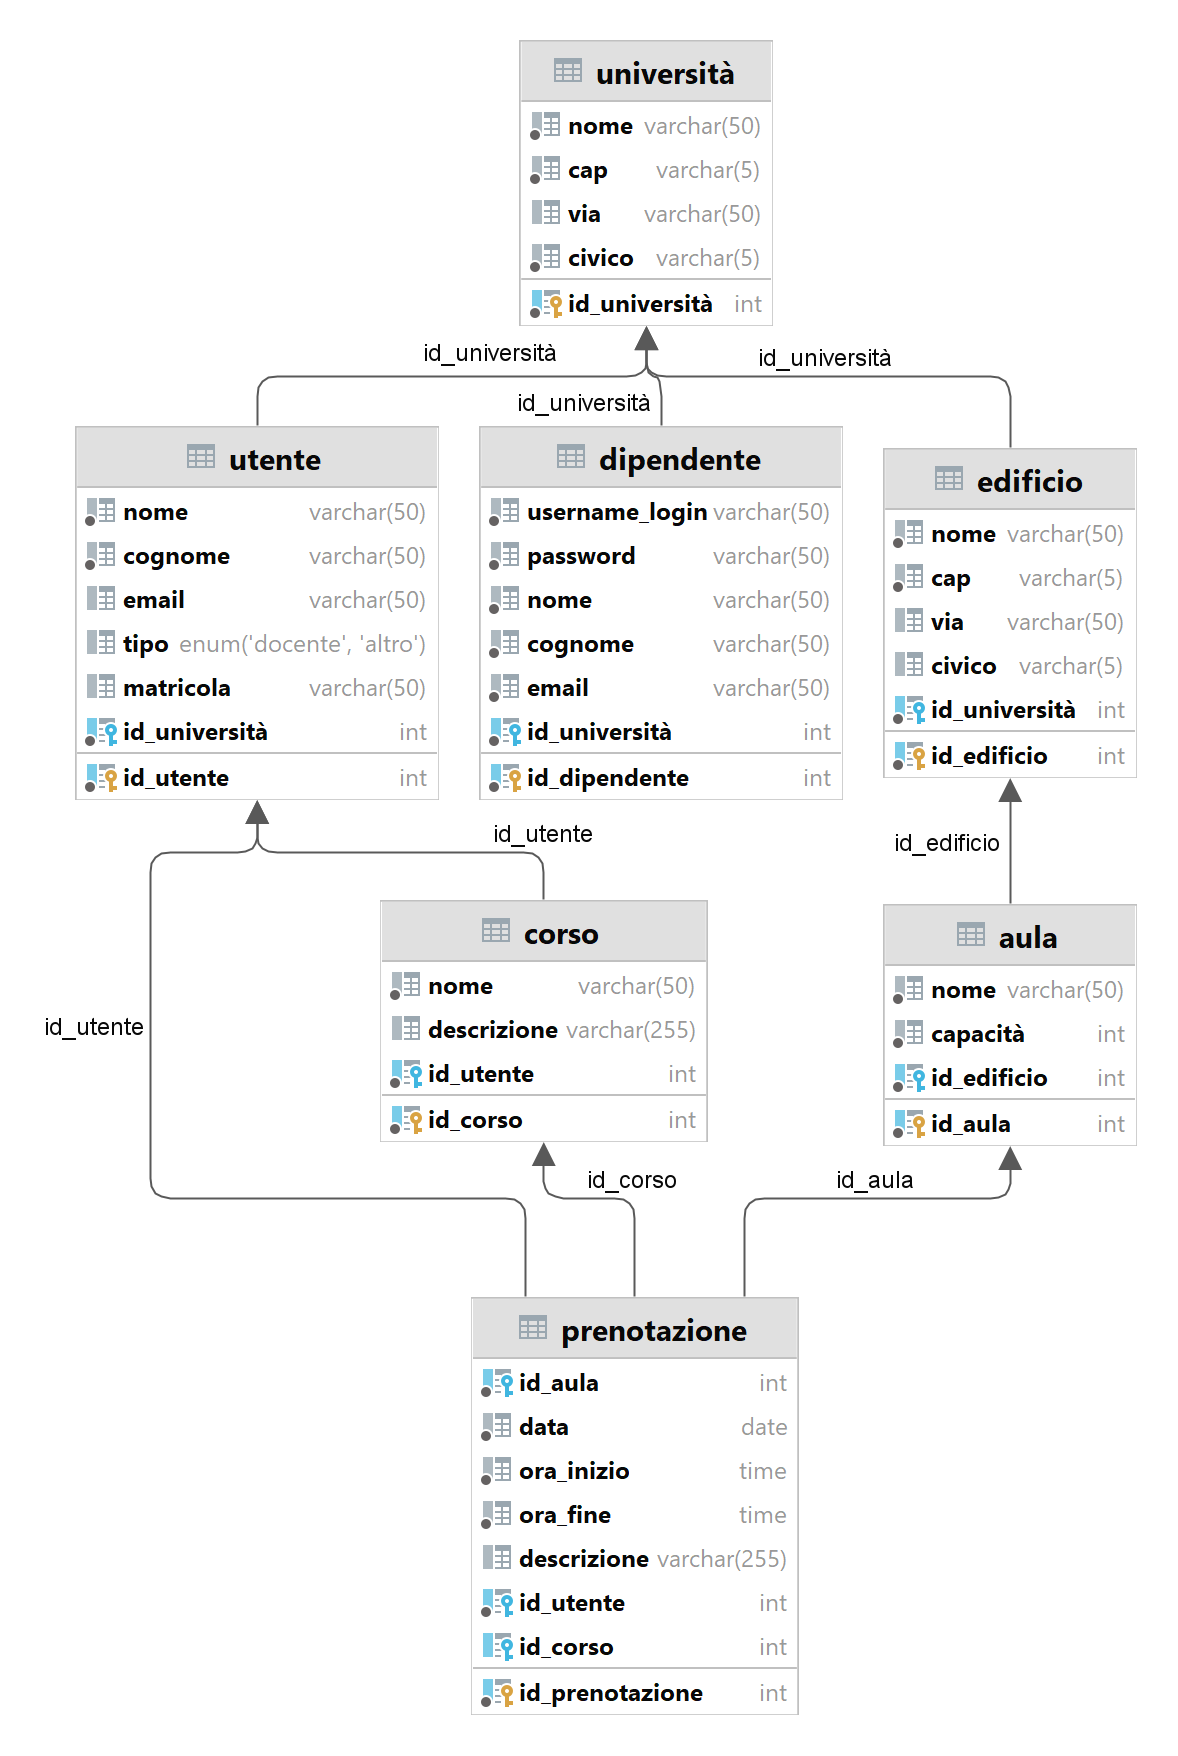
\includegraphics[width=.62\textwidth]{logico.png}
  \caption{Schema logico}
\end{figure}





\section{Realizzazione delle operazioni}

In questa sezione verranno descritti i Trigger, le Stored Procedures e viste usati nel progetto. Il loro codice è indicato in un file a parte.

\subsection{Trigger}

\subsubsection*{\texttt{controllo\_associazione\_corsi\_docenti}}

Questo trigger è progettato per essere eseguito prima dell'inserimento di una riga nella tabella "Corsi". Il suo scopo è verificare se l'utente associato al corso ha il ruolo di "Docente" nel sistema. Se l'utente non ha il ruolo corretto, viene generata un'eccezione con un messaggio di errore specifico, impedendo l'inserimento della riga nella tabella "Corsi". Questo trigger assicura che solo gli utenti con il ruolo corretto possano essere associati a un corso, garantendo la correttezza dei dati nel database.\\

\subsubsection*{\texttt{controllo\_piu\_prenotazioni\_per\_utente}}

Questo trigger viene eseguito prima dell'inserimento di una nuova riga nella tabella "Prenotazioni". Controlla se l'utente ha già effettuato una prenotazione per lo stesso giorno e se l'intervallo di ore della nuova prenotazione si sovrappone con altre prenotazioni attive dell'utente. Se viene rilevata una sovrapposizione, viene generata un'eccezione.


\subsubsection*{\texttt{controllo\_piu\_università\_per\_edificio}}
Questo trigger viene eseguito prima dell'inserimento di una nuova riga nella tabella "Edifici". Controlla se l'edificio è già associato a un'altra università. Se viene rilevata un'associazione esistente, viene generata un'eccezione.

\subsubsection*{\texttt{controllo\_piu\_edifici\_per\_aula}}

Questo trigger viene eseguito prima dell'inserimento di una nuova riga nella tabella "Aule". Controlla se l'aula è già associata a un altro edificio. Se viene rilevata un'associazione esistente, viene generata un'eccezione.

\subsubsection*{\texttt{controllo\_universita\_utente\_aula}}

Questo trigger viene eseguito prima di inserire una nuova riga nella tabella "Prenotazioni". Recupera l'id\_universita dell'aula associata alla prenotazione (attraverso l'associazione tra le tabelle Aula, Edificio e Prenotazioni) e l'id\_universita dell'utente associato alla prenotazione. Se i due id\_universita non combaciano, viene generato un errore con il messaggio specificato. In caso contrario, l'inserimento della riga nella tabella "Prenotazioni" procede normalmente.

\subsubsection*{Considerazione sul vincolo delle prenotazioni sovrapposte}
Si potrebbe implementare un trigger per controllare la disponibilità dell'aula prima di inserire la prenotazione nella tabella delle prenotazioni. Tuttavia ciò non serve perché questo controllo è già stato implementato nella stored procedure che si occupa di registrare la prenotazione nella base di dati.




\subsection{Stored Procedures}

Si precisa che sotto ogni descrizione si indicano anche i nomi dei parametri per invocare queste Stored Procedures attraverso l'applicazione indicata nel paragrafo "Demo del progetto" del presente documento. 

\subsubsection*{\texttt{AuleDisponibili()}}


La stored procedure "\texttt{AuleDisponibili()}" restituisce l'elenco delle aule disponibili in una data ora e giorno, filtrate in base alla loro capacità, fornendo una soluzione efficiente e automatizzata per la pianificazione delle attività scolastiche e universitarie.

\subsubsection*{Nomi dei parametri}

\texttt{nomeUniversita, capacita, data, oraInizio, oraFine}

\subsubsection*{\texttt{ElencoPrenotazioniAula()}}

La stored procedure "\texttt{ElencoPrenotazioniAula()}" restituisce un elenco dettagliato delle prenotazioni di un'aula in un determinato intervallo di tempo. La procedura richiede come input la data di inizio e la data di fine dell'intervallo temporale, insieme all'ID dell'aula di interesse.

\subsubsection*{Nomi dei parametri}

\texttt{dataInizio, dataFine, aulaID}

\subsubsection*{\texttt{ElencoPrenotazioniUtente()}}

La stored procedure "\texttt{ElencoPrenotazioniUtente()}" prende in input il nome di un utente (indifferente se docente o altro) e due date, e restituisce tutte le prenotazioni di aule effettuate dal docente nell'intervallo di tempo specificato.

\subsubsection*{Nomi dei parametri}

\texttt{dataInizio, dataFine, utenteID}


\subsubsection*{\texttt{AnnullaPrenotazione()}}

La stored procedure "\texttt{AnnullaPrenotazione()}" consente di annullare una prenotazione esistente nel sistema. Prende in input l'ID della prenotazione da annullare e esegue le seguenti operazioni:

\begin{enumerate}
    \item Verifica se la prenotazione esiste nel database.
    \item Se la prenotazione viene trovata, elimina la corrispondente riga dalla tabella delle prenotazioni.
    \item Restituisce un messaggio di conferma indicando che la prenotazione è stata annullata con successo.

\end{enumerate}

La stored procedure "AnnullaPrenotazione()" è utile per gestire situazioni in cui un'aula non è più disponibile per una prenotazione effettuata in precedenza, consentendo agli utenti di liberare l'aula e rendendola nuovamente disponibile per altre prenotazioni.


\subsubsection*{Nomi dei parametri}

\texttt{prenotazioneID}

\subsubsection*{\texttt{PrenotaAula()}}

La stored procedure "\texttt{PrenotaAula()}" consente di effettuare una prenotazione di un'aula per un determinato corso presso un'istituzione accademica. Accetta come parametri di input l'ID dell'aula, la data, l'ora di inizio e di fine della prenotazione, la descrizione del corso, l'ID del corso e l'ID dell'utente che effettua la prenotazione.\\

All'interno della procedura, vengono eseguiti controlli per verificare la disponibilità dell'aula nel periodo specificato. Se l'aula è disponibile, viene creata una nuova riga nella tabella delle prenotazioni con i dettagli forniti. In caso di conflitto con altre prenotazioni esistenti, la procedura restituisce un messaggio di errore appropriato.\\

Inoltre, viene controllata l'esistenza delle righe corrispondenti ai valori specificati di AulaID, UtenteID e CorsoID nelle tabelle "aule", "utenti" e "corsi" rispettivamente, prima di eseguire l'inserimento di una nuova riga nella tabella "prenotazioni". Ciò è importante per garantire la consistenza dei dati nel database. Senza questa verifica, potrebbero verificarsi problemi di consistenza se si inseriscono righe nella tabella "prenotazioni" che fanno riferimento a valori di AulaID, UtenteID o CorsoID non esistenti nelle tabelle corrispondenti.\\

La stored procedure "PrenotaAule" contribuisce a semplificare il processo di prenotazione delle aule, garantendo che le prenotazioni siano gestite correttamente e prevenendo sovrapposizioni o doppie prenotazioni.

\subsubsection*{Nomi dei parametri}

\texttt{aulaID, data, oraInizio, oraFine, descr, corsoID, utenteID}


\subsection{Viste}

\subsubsection*{\texttt{ElencoPrenotazioni}}

La vista "\texttt{ElencoPrenotazioni}" fornisce una visualizzazione dei dettagli delle prenotazioni effettuate per le aule.\\

La vista è costruita utilizzando diverse operazioni di join tra le tabelle. Questo consente di ottenere un'unica tabella che combina le informazioni necessarie per visualizzare in modo chiaro e dettagliato le prenotazioni delle aule, inclusi i relativi contesti (aula, edificio, università), il corso associato (se presente) e il responsabile della prenotazione.


\subsubsection*{\texttt{ElencoAule}, \texttt{ElencoEdifici}  e \texttt{ElencoUniversità}}

La vista "\texttt{ElencoAule}" fornisce un elenco delle aule disponibili, insieme alle informazioni sull'edificio e sull'università a cui appartengono. Ogni riga della vista rappresenta un'aula e include il nome dell'aula. il nome dell'edificio in cui si trova l'aula, il nome dell'università a cui l'edificio e l'aula appartengono, l'indirizzo completo dell'edificio, ottenuto concatenando via, civico e cap.\\

Semplificando la vista "\texttt{ElencoAule}", è possibile anche ottenere le viste "\texttt{ElencoEdifici}" e "\texttt{ElencoUniversità}". Nella vista "\texttt{ElencoEdifici}" si visualizza il nome dell'edificio, l'università d'appartenenza e l'indirizzo. Invece nel caso "\texttt{ElencoUniversità}" si visualizza il nome dell'Università e l'indirizzo della sede principale.\\


Questa vista fornisce un modo pratico per ottenere un elenco completo delle aule disponibili nel sistema, insieme alle informazioni sull'edificio e sull'università di appartenenza. È particolarmente utile per scopi di visualizzazione e reportistica, consentendo agli utenti di ottenere rapidamente una panoramica delle aule e delle relative posizioni.

\subsubsection*{\texttt{ElencoDocenti} e \texttt{ElencoNonDocenti}}

La vista "\texttt{ElencoDocenti}" fornisce un elenco dei docenti presenti nel sistema, includendo i loro nomi, cognomi, indirizzi email, matricole e l'università a cui sono affiliati. Questa vista permette di ottenere un rapido accesso alle informazioni essenziali sui docenti presenti nel sistema.\\

In maniera del tutto analoga è stata creata la vista "\texttt{ElencoNonDocenti}" che invece fornisce un elenco degli utenti con una tipologia "Altro".

\subsubsection*{\texttt{ElencoCorsi}}

Questa vista elenca i corsi disponibili nel sistema, includendo il nome del corso, la sua descrizione, il nome completo del docente che lo tiene (concatenando nome e cognome) e il nome dell'università in cui il corso è tenuto. È possibile utilizzare questa vista per ottenere una visione completa dei corsi offerti, comprensiva di informazioni sul docente e sull'università associata.

\subsubsection*{\texttt{ElencoDipendenti}}
Questa vista fornisce un elenco dei dipendenti dell'università, includendo il nome, il cognome, l'email e il nome dell'università di appartenenza. Il campo password è escluso dalla vista per proteggere la privacy dei dipendenti.



\section{Demo del progetto}
È disponibile una demo con una app Python (Flask) che serve una semplice applicazione web che realizza alcune funzioni sql descritte nel progetto. Viene utilizzato un container Docker e, per semplicità, non è stata implementato il Backend per la segreteria.\\

La decisione di non implementare il backend per la segreteria nella demo è principalmente motivata dalla complessità aggiuntiva che comporta la gestione dei dati sensibili e la sicurezza del sistema. L'implementazione di un sistema di crittografia adeguato per i campi sensibili del database, come password o informazioni personali, richiede una conoscenza avanzata della crittografia e delle best practice di sicurezza.\\

In questa applicazione si evita totalmente con le Stored Procedures di fare concatenazione di stringhe perché potrebbe comportare a delle SQL injections. Per quanto riguarda invece le viste, viene effettuato un controllo sull'input.\\

Vengono utilizzate le transazioni per eseguire le stored procedure. Sono importanti soprattutto per quelle che comportano un cambiamento dello stato del database (\texttt{PrenotaAula()} e \texttt{AnnullaPrenotazione()}). Le transazioni sono un meccanismo fondamentale per garantire l'integrità e la coerenza dei dati all'interno di un database. Si ricorda in particolare che sono fondamentali per garantire che le modifiche siano eseguite in modo atomico, coerente, isolato e durevole, seguendo il principio ACID.

Si specifica infine che in realtà il database ha una piccola differenza rispetto a quello descritto nel documento: per motivi legati di codifica si sceglie di usare parole senza la a accentata (\texttt{à}). Viene sostituita con la a normale senza l'accento (\texttt{a}).

\subsection{Funzionamento}

L'applicazione sviluppata ha lo scopo di gestire richieste POST (nel caso delle stored procedure) oppure GET (nel caso delle viste) e restituire una risposta JSON in base al percorso URL specificato.\\

Se il percorso URL inizia con \texttt{/sp/} seguito dal nome di una stored procedure, l'applicazione eseguirà la stored procedure corrispondente utilizzando i parametri forniti nel corpo della richiesta in formato JSON (i nomi dei parametri da indicare sono nel paragrafo "Stored Procedures"). I risultati della stored procedure verranno quindi restituiti come una risposta JSON.\\

In maniera analoga, se il percorso URL inizia con \texttt{/v/} seguito dal nome di una vista, l'applicazione eseguirà una query di selezione \texttt{SELECT * FROM nomeVista} per ottenere i dati dalla vista specificata. I risultati della query verranno restituiti come una risposta JSON.

\subsection{Esempi d'uso}

Per usare questa applicazione si può utilizzare l'applicativo cURL (negli esempi è usata la versione per Windows, la sintassi della versione per sistemi operativi basati su kernel GNU/Linux è leggermente diversa).

\lstset{
basicstyle=\ttfamily,
breaklines=true,
columns=fullflexible,
frame=single,
showstringspaces=false
}

\subsubsection*{Esempio 1}
\begin{lstlisting}[language=bash]
curl -X POST -H "Content-Type: application/json" -d "{\"dataInizio\":\"2010-05-16\",\"dataFine\":\"2023-05-18\",\"aulaID\":2}" http://localhost:5000/sp/ElencoPrenotazioniAula
\end{lstlisting}

\subsubsection*{Esempio 2}
\begin{lstlisting}[language=bash]
curl http://localhost:5000/v/ElencoDocenti
\end{lstlisting}



\section{Dichiarazione finale}

Il progetto (inteso come questo documento e tutti i file nel repository github) è stato svolto da me in completa autonomia.

\bigskip

\begin{flushleft}
Giovanni de Maria\\
IN0500952\\
\textit{Trieste, \today}
\end{flushleft}
\end{document}